\section{Path Planning - Laparoscopic tool manipulation}

\textbf{Path Planning} is a geometric problem, where it is desired to find a path from a starting point to a goal point and also satisfying a set of constraints, such as: 
restricting the solutions inside the robot's configuration space, avoiding obstacles in the task space, avoiding singularity points and respecting the robot's 
joint limits.

The biggest challenge in manipulating a laparoscopic tool with a robot is overcoming the \textbf{fulcrum effect} problem. This is also one of the reasons that 
robotic assisted surgery replaced the traditional laparoscopic procedures. The fulcrum effect means that the surgeon's hand motions are inverted and scaled 
with respect to the Remote Center of Motion point, which lies approximately on the center of the incision. Apart from the scaling and inversion, laparoscopic 
procedures add an additional motion constraint that demands at each time one point of the laparoscopic tool to coincide with the RCM point.

\subsection{Tool pose}

\begin{center}
\begin{figure}[H]
\centering
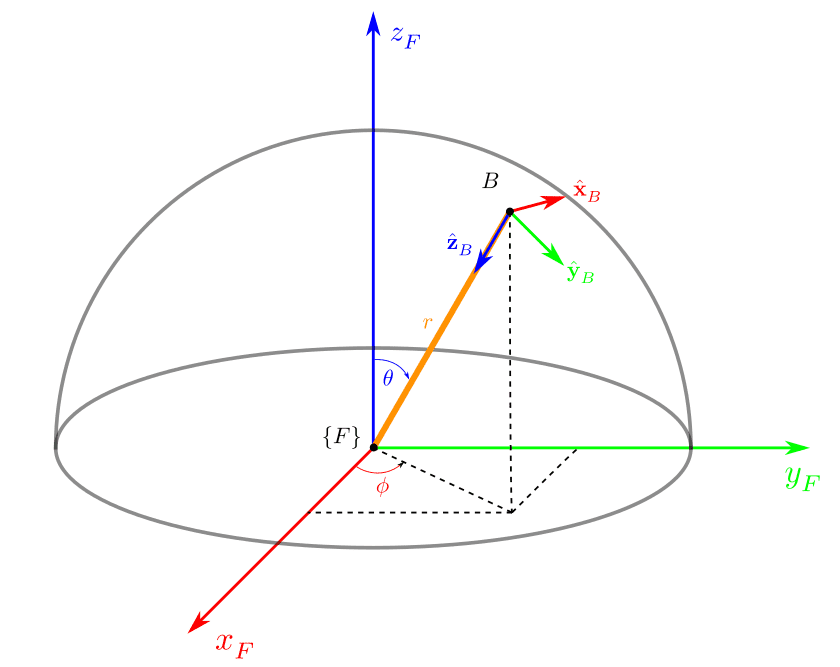
\includegraphics[width=12cm]{images/fulcrum-space.png}\\
\caption{Tool pose at target point $B$ calculated with respect to Fulcrum's reference frame $\lbrace F \rbrace$}
\end{figure}
\end{center}

The laparoscopic tool pose is given by the position and orientation vectors at target point $B$ with respect to the coordinate frame $\lbrace F \rbrace$.
The pose is given by the following transformation matrix
\[
{}^{F}T_B = \begin{bmatrix}
{}^{F}R_B & {}^{F}\mathbf{p}^{}_B \\
\mathbf{0} & 1 \\
\end{bmatrix}
\;\; where \;\;
{}^{F}R_B = \begin{bmatrix}
\hat{\mathbf{x}}^{}_B & \hat{\mathbf{y}}^{}_B & \hat{\mathbf{z}}^{}_B \\
\end{bmatrix}
\]

\begin{equation}
\hat{\mathbf{x}}^{}_B = \hat{\mathbf{θ}} = cos(θ)cos(φ)\hat{\mathbf{x}}^{}_F + cos(θ)sin(φ)\hat{\mathbf{y}}^{}_F - sin(θ)\hat{\mathbf{z}}^{}_F
= \begin{bmatrix}
cos(θ)cos(φ) \\
cos(θ)sin(φ) \\
- sin(θ) \\
\end{bmatrix}
\end{equation}

\begin{equation}
\hat{\mathbf{y}}^{}_B = \hat{\mathbf{φ}} = -sin(φ)\hat{\mathbf{x}}^{}_F + cos(φ)\hat{\mathbf{y}}^{}_F
= \begin{bmatrix}
-sin(φ) \\
cos(φ) \\
0 \\
\end{bmatrix}
\end{equation}

\begin{equation}
\hat{\mathbf{z}}^{}_B = - \hat{\mathbf{r}} = - (sin(θ)cos(φ)\hat{\mathbf{x}}^{}_F + sin(θ)sin(φ)\hat{\mathbf{y}}^{}_F + cos(θ)\hat{\mathbf{z}}^{}_F)
= \begin{bmatrix}
-sin(θ)cos(φ) \\
-sin(θ)sin(φ) \\
-cos(θ) \\
\end{bmatrix}
\end{equation}

The position of the point $B$ is given in spherical coordinates by:
\begin{itemize}
	\item $r=ρ$ : outside penetration of laparoscopic tool
	\item $θ=β$ : altitude angle
	\item $φ=α$ : orientation angle
\end{itemize}
thus the position with respect to the coordinate frame $\lbrace F \rbrace$ is given by
\begin{equation}
{}^{F}\mathbf{p}^{}_B = \begin{bmatrix}
ρsin(β)cos(α) \\
ρsin(β)sin(α) \\
ρcos(β) \\
\end{bmatrix} = ρ \hat{\mathbf{r}}
\end{equation}

The above goal point must be the same as the $TCP$ point of the robot's end-effector. This means, that this pose must be converted with respect to the robot's reference frames.
\[
{}^{U}T^{}_{TCP} = {}^{U}T^{}_{B}
\]
\[
{}^{U}T^{}_{0} \; {}^{0}T^{}_{7} \; {}^{7}T^{}_{TCP} = {}^{U}T^{}_{F} \; {}^{F}T^{}_{B}
\]
\begin{equation}
{}^{0}T^{}_{7} = {}^{U}T^{-1}_{0} \; {}^{U}T^{}_{F} \; {}^{F}T^{}_{B} \; {}^{7}T^{-1}_{TCP}
\end{equation}

\subsection{Pivoting motion with respect to Fulcrum Point}
\label{subsection:pivot-motions}

On this section, some basic pivoting trajectories around the fulcrum point, are presented. In all of the following three example pivoting motions, we have made 
the assumption that the position and orientation of the ${F}$ reference frame is precisely known, which is however not applicable in real-life scenarios ()

\subsubsection{Circular path of tool tip}

\begin{center}
\begin{figure}[H]
\centering
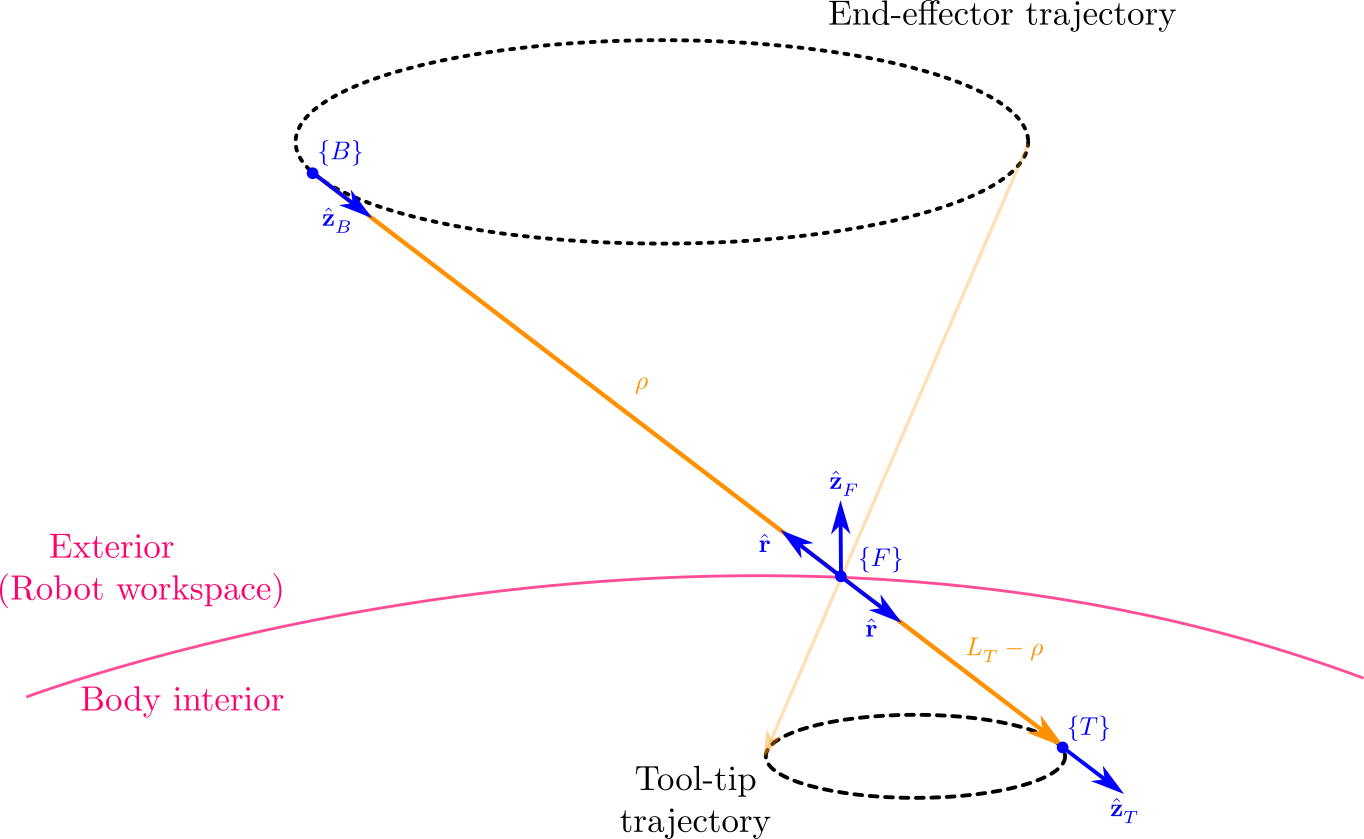
\includegraphics[width=12cm]{images/circular-trajectory-wrt-fulcrum.png}\\
\caption{Circular trajectory of tool tip with respect to Fulcrum reference frame}
\end{figure}
\end{center}

To generate a circular trajectory for the pivot movement we must specify the center of the circle 
and a vector whose magnitude is the radius of the circle and it’s direction gives the orientation 
of the plane that the circle lies at. The simplest case of a circular trajectory is the one, 
whose circle lies in a plane parallel to the xy plane.


We first consider the motion of the laparoscopic tool tip on a circle parallel to a z-plane, with respect to the $\lbrace F \rbrace$ coordinate frame.
\begin{equation}
(x^{}_{F} - x^{}_{F0})^2 + (y^{}_{F} - y^{}_{F0})^2 = r_0^2, \;\; z^{}_{F} = z^{}_{F0}
\end{equation}
It's often more convenient to express trajectories in a parametric form, which makes it easier to calculate all the waypoints of the trajectory
\begin{equation}
\begin{cases}
x^{}_{F} = r_0cos(2πs) + x^{}_{F0} \\
y^{}_{F} = r_0sin(2πs) + y^{}_{F0} \\
z^{}_{F} = z^{}_{F0}
\end{cases} ,
\;\;
s \in [0, 1]
\end{equation}

After having calculated the cartesian coordinates we can calculate the spherical coordinates as follows

\begin{equation}
\label{eqns:cartesian-to-spherical}
\begin{cases}
r = \sqrt{x^{2}_{F} + y^{2}_{F} + z^{2}_{F}} \\
θ = atan2 \left( \sqrt{x^{2}_{F} + y^{2}_{F}}, z^{}_{F} \right) \\
φ = atan2(y^{}_{F}, x^{}_{F})
\end{cases}
\end{equation}

\subsubsection{Circular arc path of tool tip}

To generate a circular arc trajectory for a pivot motion we must specify the same parameters as 
in the circular trajectory as well as the length of the arc or the total angle of the arc 
section.


\subsubsection{Line segment path of tool tip}

\begin{center}
\begin{figure}[H]
\centering
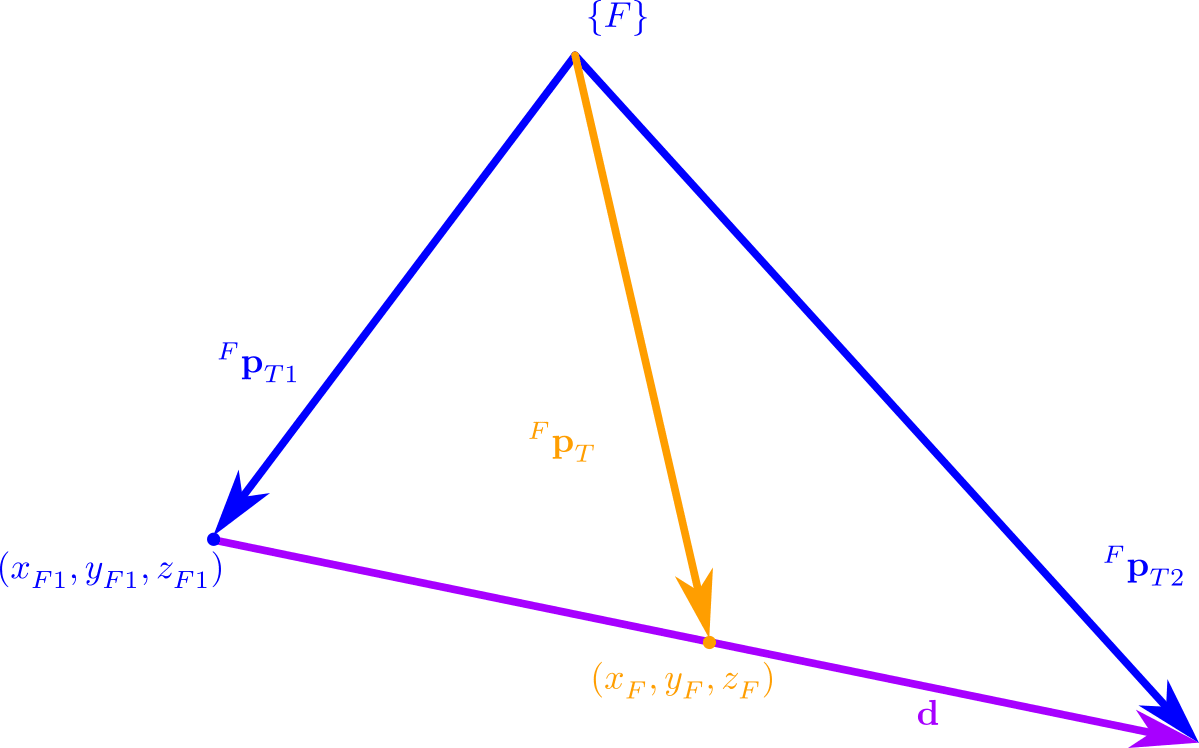
\includegraphics[width=10cm]{images/line-segment-trajectory-wrt-fulcrum.png}\\
\caption{Line segment trajectory of tool tip with respect to Fulcrum reference frame}
\end{figure}
\end{center}
\[
\mathbf{d} = {}^{F}\mathbf{p}^{}_{T2} - {}^{F}\mathbf{p}^{}_{T1} = [l, m, n]^\top
\]
\[
{}^{F}\mathbf{p}^{}_{T} = [x^{}_{F}, y^{}_{F}, z^{}_{F}]^\top
\]
\[
{}^{F}\mathbf{p}^{}_{T} = {}^{F}\mathbf{p}^{}_{T1} + s\mathbf{d}
\]
\[
s = \frac{x^{}_{F} - x^{}_{F1}}{l} = \frac{y^{}_{F} - y^{}_{F1}}{m} = \frac{z^{}_{F} - z^{}_{F1}}{n} \;\; s \in [0, 1]
\]

\begin{equation}
\begin{cases}
x^{}_{F} = sl + x^{}_{F1} = (1-s)x^{}_{F1} + sx^{}_{F2} \\
y^{}_{F} = sm + y^{}_{F1} = (1-s)y^{}_{F1} + sy^{}_{F2} \\
z^{}_{F} = sn + z^{}_{F1} = (1-s)z^{}_{F1} + sz^{}_{F2}
\end{cases}
\end{equation}

After having calculated the cartesian coordinates we can calculate the spherical coordinates using the \ref{eqns:cartesian-to-spherical} equations.

The line segment trajectory of tool tip, as analysed in this section needs no implementation as 
it is already implemented in the ROS MoveIt library and can be used by calling the method 
\textbf{computeCartesianPath}.

\subsubsection{Cubic Spline path of tool tip}

A useful mathematical tool to construct a smooth curve that visits every point from a given set of waypoints are \textbf{cubic splines}. A cubic spline is 
constructed using smaller curves that are described by a polynomial of 3rd order. Let $\left\lbrace \mathbf{P}_0, \mathbf{P}_1, \ldots , \mathbf{P}_n \right\rbrace$ 
be a set of waypoints, where each point has coordinates $\mathbf{P}_i = [x_i, y_i, z_i]^\top$. Then between each 2 points a cubic 
polynomial can be constructed (one for each coordinate, 3 in total). The following equations are for the $x$-coordinate and in the exact same way one can 
calculate the cubic polynomials for the $y,z$ coordinates as well. For each pair of waypoints we want to calculate the following cubic polynomial
\begin{equation}
\label{cubic-polynomial}
x_i(s) = a_i(s-s_i)^3 + b_i(s-s_i)^2 + c_i(s-s_i) + d_i, \hspace{3em} s_i \leqslant s \leqslant s_{i+1}
\end{equation}

The polynomial in equation \ref{cubic-polynomial} has four unknowns which means that four additional equations are needed to get a unique solution and fully 
define the polynomial. These equations can be formed using the boundary conditions for the first and last point of each curve.
\begin{equation}
x_i(s_i) = x_i
\end{equation}
\begin{equation}
x_i(s_{i+1}) = x_{i+1}
\end{equation}
\begin{equation}
\dot{x}_i(s_i) = \dot{x}_i
\end{equation}
\begin{equation}
\dot{x}_i(s_{i+1}) = \dot{x}_{i+1}
\end{equation}

First we solve for $c_i$ and $d_i$, which can easily be calculated as follows
\begin{equation}
\label{di-eq}
d_i = x_i(s_i) = x_i
\end{equation}
and by taking the derivative of \ref{cubic-polynomial}, we can calculate $c_i$
\begin{equation}
\label{cubic-polynomial-first-derivative}
\dot{x}_i(s_i) = 3a_i(s-s_i)^2 + 2b_i(s-s_i) + c_i
\end{equation}
\begin{equation}
\label{ci-eq}
c_i = \dot{x}_i(s_i) = \dot{x}_i
\end{equation}

By substituting $s = s_{i+1}$ in \ref{cubic-polynomial} and \ref{cubic-polynomial-first-derivative}, by using equations \ref{ci-eq}, \ref{di-eq} and if 
we set $σ = s_{i+1}-s_i$ for brevity, we get the following two equations
\begin{equation}
\label{xi1}
x_{i+1} = x_i(s_{i+1}) = a_i σ^3 + b_i σ^2 + c_i σ + x_i
\end{equation}
and
\begin{equation}
\label{xdi1}
\dot{x}_{i+1} = \dot{x}_i(s_{i+1}) = 3a_i σ^2 + 2b_i σ + \dot{x}_i
\end{equation}

By multiplying \ref{xdi1} by $σ$ and \ref{xi1} by $-3$ and add them together we get
\[
\dot{x}_{i+1}σ - 3x_{i+1} = -b_iσ^2 -2\dot{x}_iσ - 3x_i
\]
\begin{equation}
b_i = \frac{1}{σ^2} (3x_{i+1} -3x_i - \dot{x}_{i+1}σ - 2\dot{x}_iσ)
\end{equation}

Similarly, by multiplying \ref{xdi1} by $σ$ and \ref{xi1} by $-2$ and add them together we get
\[
\dot{x}_{i+1}σ - 2x_{i+1} = a_iσ^3 -\dot{x}_iσ - 2x_i
\]
\begin{equation}
a_i = \frac{1}{σ^3} (\dot{x}_{i+1}σ - 2x_{i+1} + \dot{x}_iσ +2x_i)
\end{equation}

\begin{center}
\begin{figure}[H]
\centering
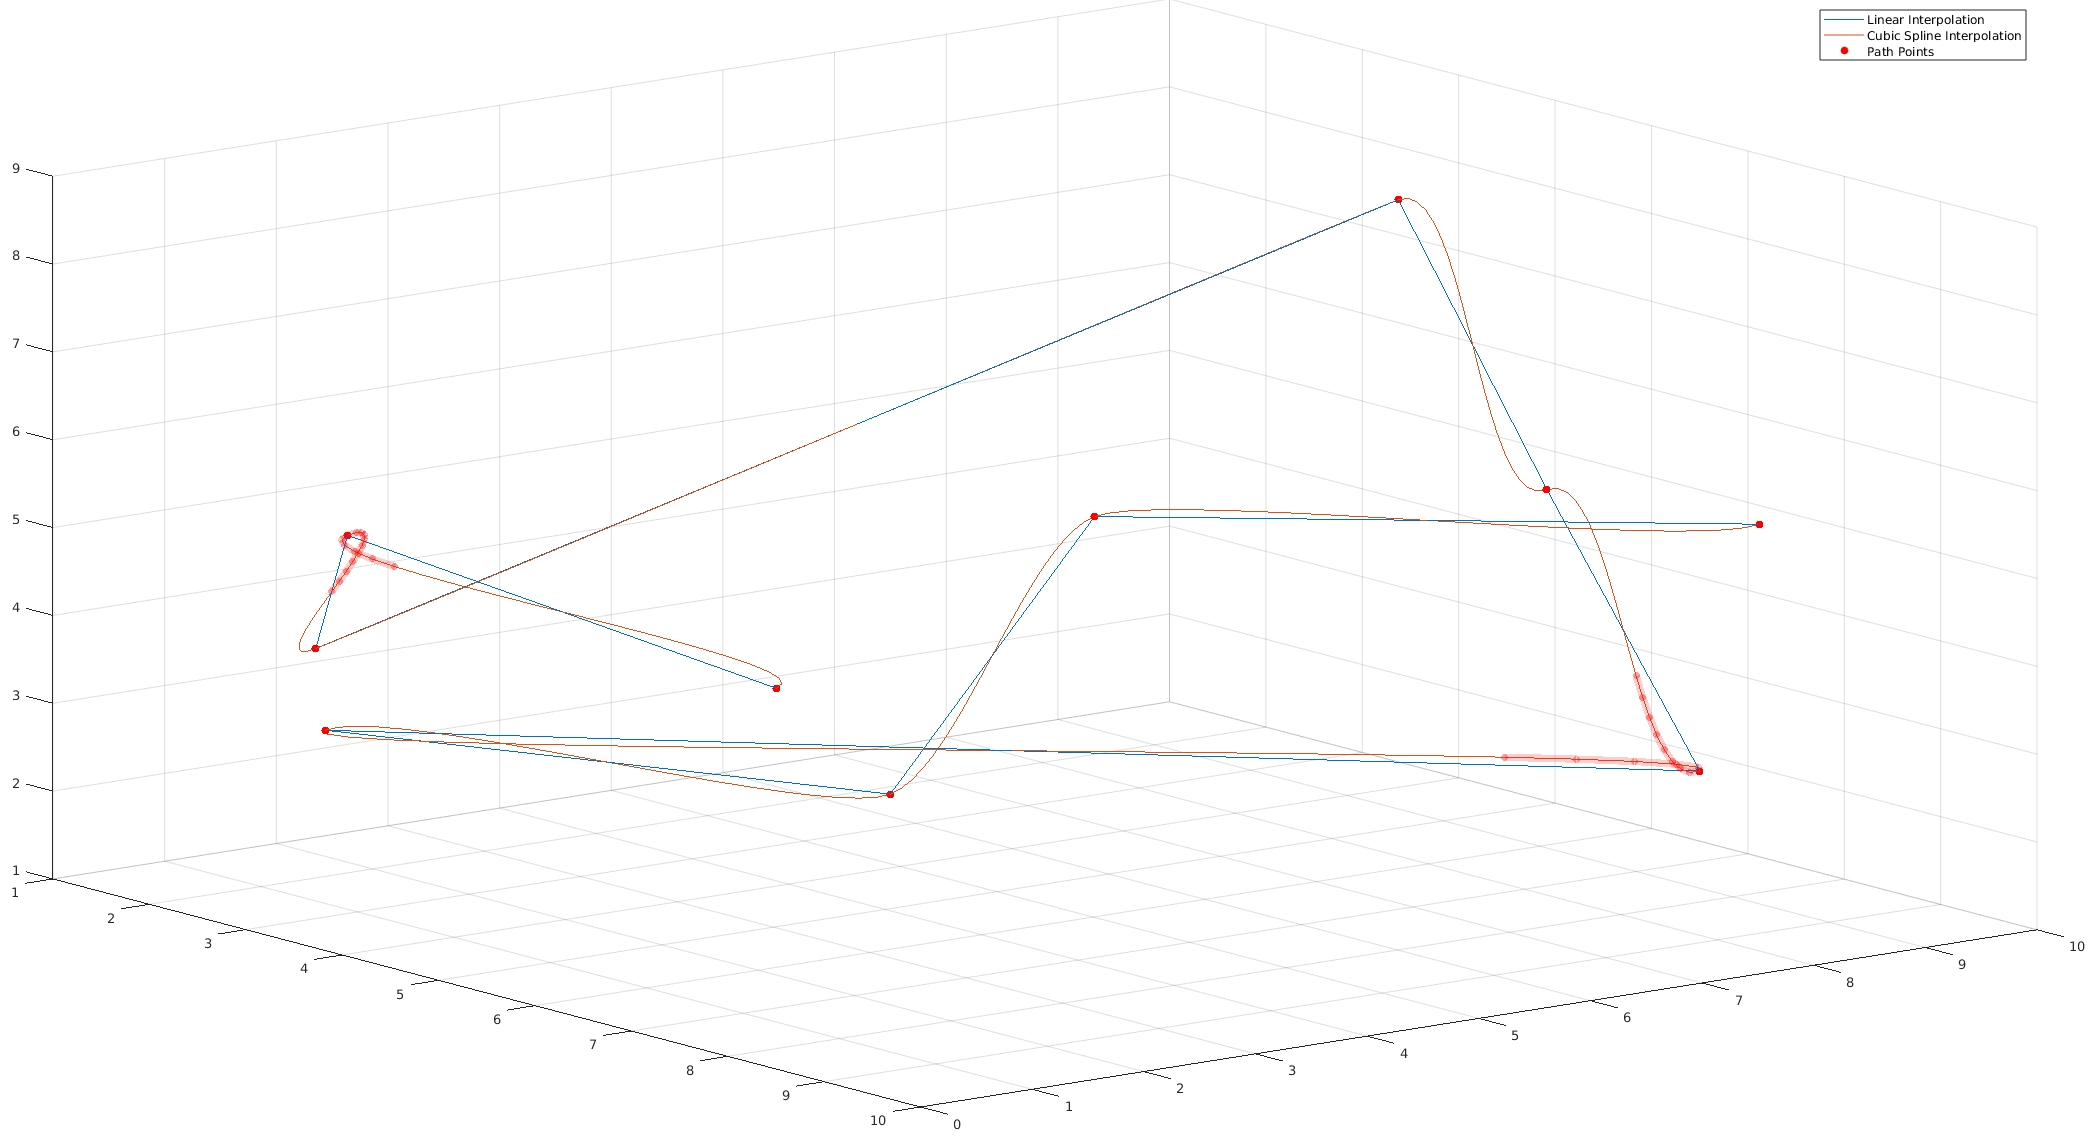
\includegraphics[width=\textwidth]{images/cubic-spline-path1.png}\\
\caption{Cubic Spline curve with 10 waypoints} 
\label{b-spline-explanation}
\end{figure}
\end{center}


\subsubsection{B-Spline path of tool tip}

The \textbf{B-Splines} are smooth curves which are constructed from \textbf{B\'ezier} curves. A B\'ezier curve is a parametric smooth curve and is a $k$-th order interpolation of $k+1$ control points.

\begin{center}
\begin{figure}[H]
\centering
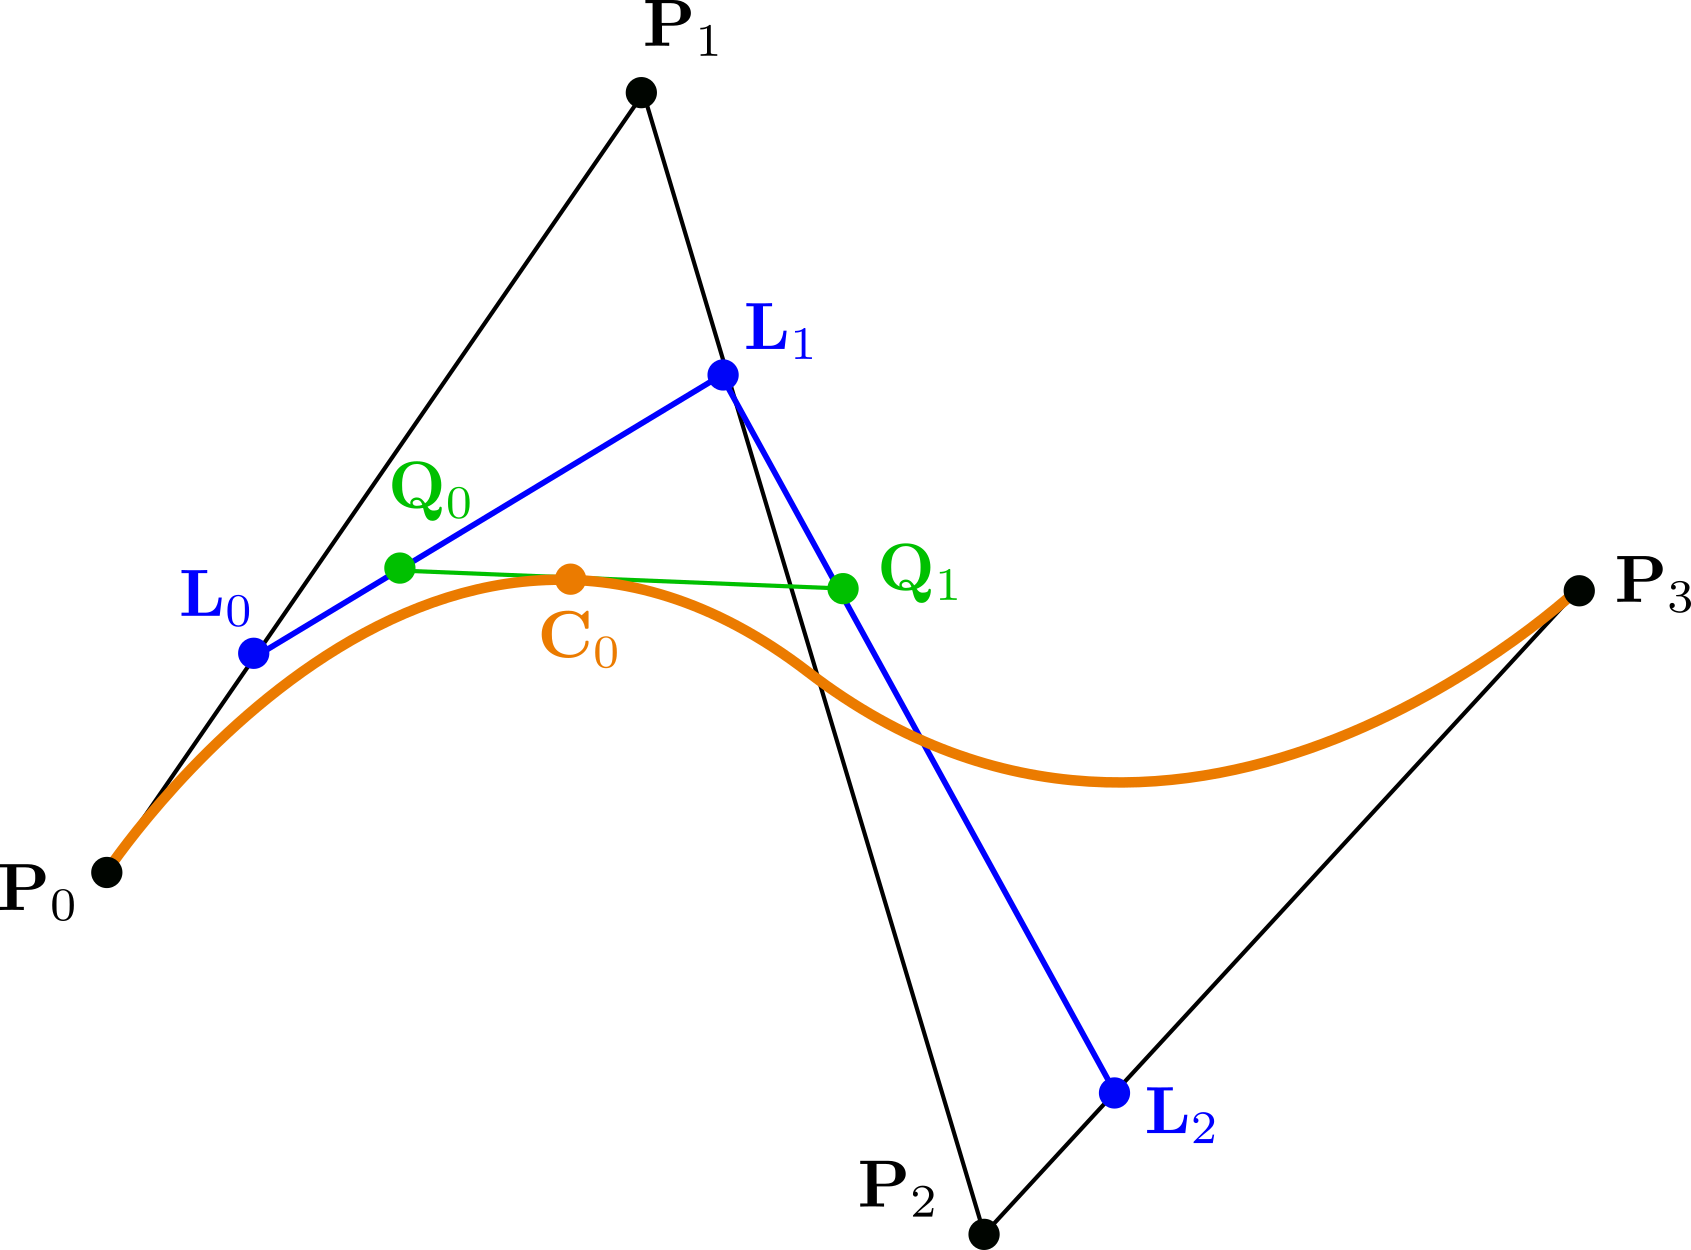
\includegraphics[width=0.5\textwidth]{images/bezier-curve.png}\\
\caption{Cubic B\'ezier curve calculated using cubic interpolation of 4 control points} 
\end{figure}
\end{center}

We first calculate the linear interpolation of the control points
\begin{equation}
\mathbf{L}_0(s) = (1-s)\mathbf{P}_0 + s\mathbf{P}_1
\end{equation}
\[
\mathbf{L}_1(s) = (1-s)\mathbf{P}_1 + s\mathbf{P}_2
\]
\[
\mathbf{L}_2(s) = (1-s)\mathbf{P}_2 + s\mathbf{P}_3
\]
The next step is to calculate the quadratic interpolation of the control points or equivalently, the linear interpolation of the previously calculated points $\mathbf{L}_0,\mathbf{L}_1,\mathbf{L}_2$
\[
\mathbf{Q}_0(s) = (1-s)\mathbf{L}_0(s) + s\mathbf{L}_1(s)
\]
\begin{equation}
\mathbf{Q}_0(s) = (1-s)^2\mathbf{P}_0 + 2(1-s)s\mathbf{P}_1 + s^2\mathbf{P}_2
\end{equation}
\[
\mathbf{Q}_1(s) = (1-s)^2\mathbf{P}_1 + 2(1-s)s\mathbf{P}_2 + s^2\mathbf{P}_3
\]
Similarly for the last step, we calculate the cubic interpolation of the control points or equivalently, the linear interpolation of the previously calculated points $\mathbf{Q}_0,\mathbf{Q}_1$
\[
\mathbf{C}_0(s) = (1-s)\mathbf{Q}_0(s) + s\mathbf{Q}_1(s)
\]
\begin{equation}
\mathbf{C}_0(s) = (1-s)^3\mathbf{P}_0 +3(1-s)^2 s\mathbf{P}_1 + 3(1-s)s^2\mathbf{P}_2 + s^3\mathbf{P}_3
\end{equation}

The cubic B\'ezier curve can also be calculated using the following more compact equation, in matrix form
\begin{equation}
\mathbf{C}_0(t) = \begin{bmatrix} \mathbf{P}_0 & \mathbf{P}_1 & \mathbf{P}_2 & \mathbf{P}_3 \end{bmatrix} 
\begin{bmatrix} 
-1 & 3 & -3 & 1 \\
3 & -6 & 3 & 0 \\
-3 & 3 & 0 & 0 \\
1 & 0 & 0 & 0
\end{bmatrix}
\begin{bmatrix}
s^3 \\ s^2 \\ s \\ 1
\end{bmatrix}
\end{equation}

A $k$-degree \textbf{B-Spline} curve defined by $n+1$ control points will consist of $n-k+1$ B\'ezier curves. For example if we want to construct a cubic B-Spline using 6 control points, then we will need to construct 
and connect together 3 B\'ezier curves.

\begin{center}
\begin{figure}[H]
\centering
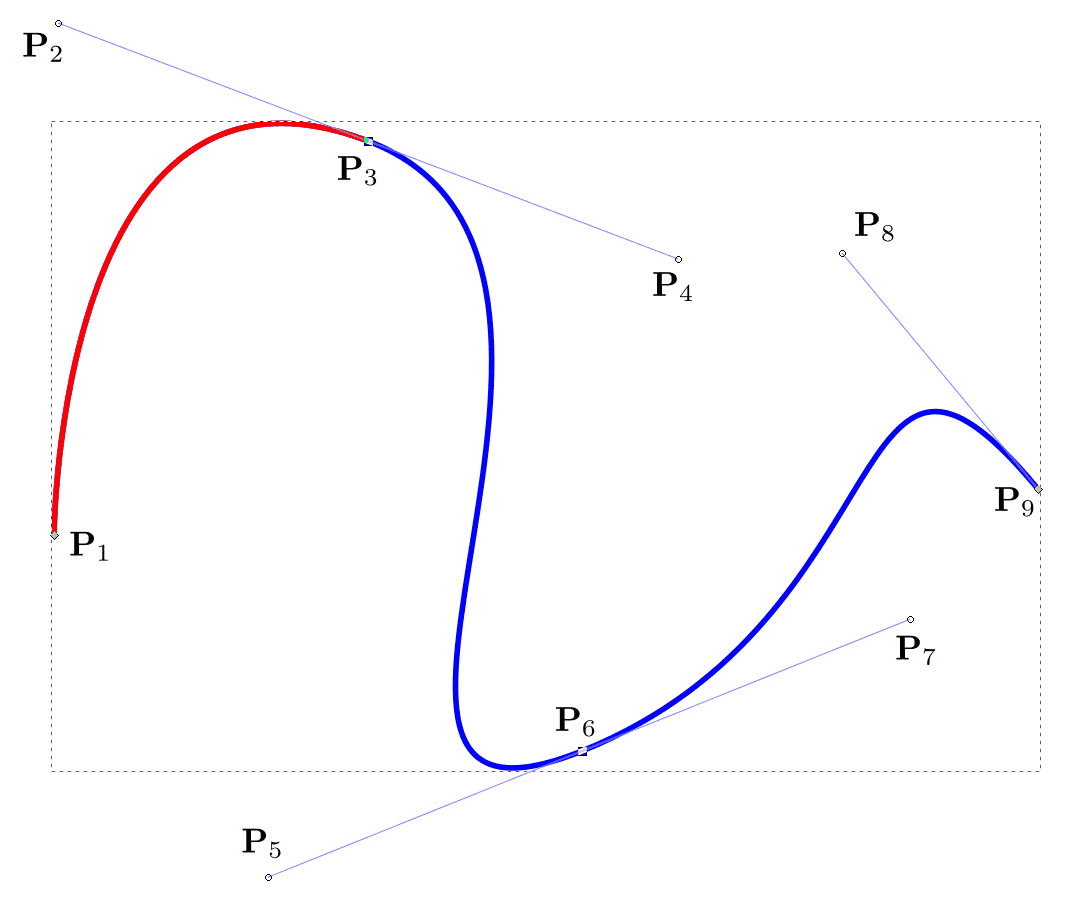
\includegraphics[width=0.6\textwidth]{images/b-spline-explanation.png}\\
\caption{B-Spline curve constructed from 3 B\'ezier curves. The first B\'ezier curve colored in red is a quadratic one and the following two are both cubic.} 
\label{b-spline-explanation}
\end{figure}
\end{center}

In most cases the B-Spline curves are constructed by starting from a quadratic B\'ezier curve, which is constructed from 3 control points and then all other 
parts of the curve are constructed from cubic B\'ezier curves, each constructed from 4 control points. As shown in figure \ref{b-spline-explanation}, the B-Spline 
curves do not pass from all control points. This means that if we have a path formed by a set of waypoints and we want the robot to pass from all of them, then 
in order to construct a B-Spline trajectory we will need additional intermediary points. The first and last points are part of the curve and the other control 
points are not. If no additional points can be calculated then the robot will not pass from all the points, which in some cases is also acceptable and useful.


\subsection{Task space analysis}

Dexterity analysis for tool's task space
\begin{equation}
\mathcal{D} = \mathcal{L}_q \mathcal{M}
\end{equation}
where
\begin{equation}
\mathcal{M} = \sqrt{det(J J^\top)}
\end{equation}
\begin{equation}
\label{joint-limit-measure}
\mathcal{L}_{q}=1-\exp\left\{-\kappa\prod_{i=1}^{n_{k}}\frac{(q_{ {i}}-q_{i,\min})(q_{i,\max}-q_{i})}{(q_{i,\max}-q_{i,\min})^{2}}\right\}
\end{equation}

\begin{center}
\begin{figure}[H]
\centering
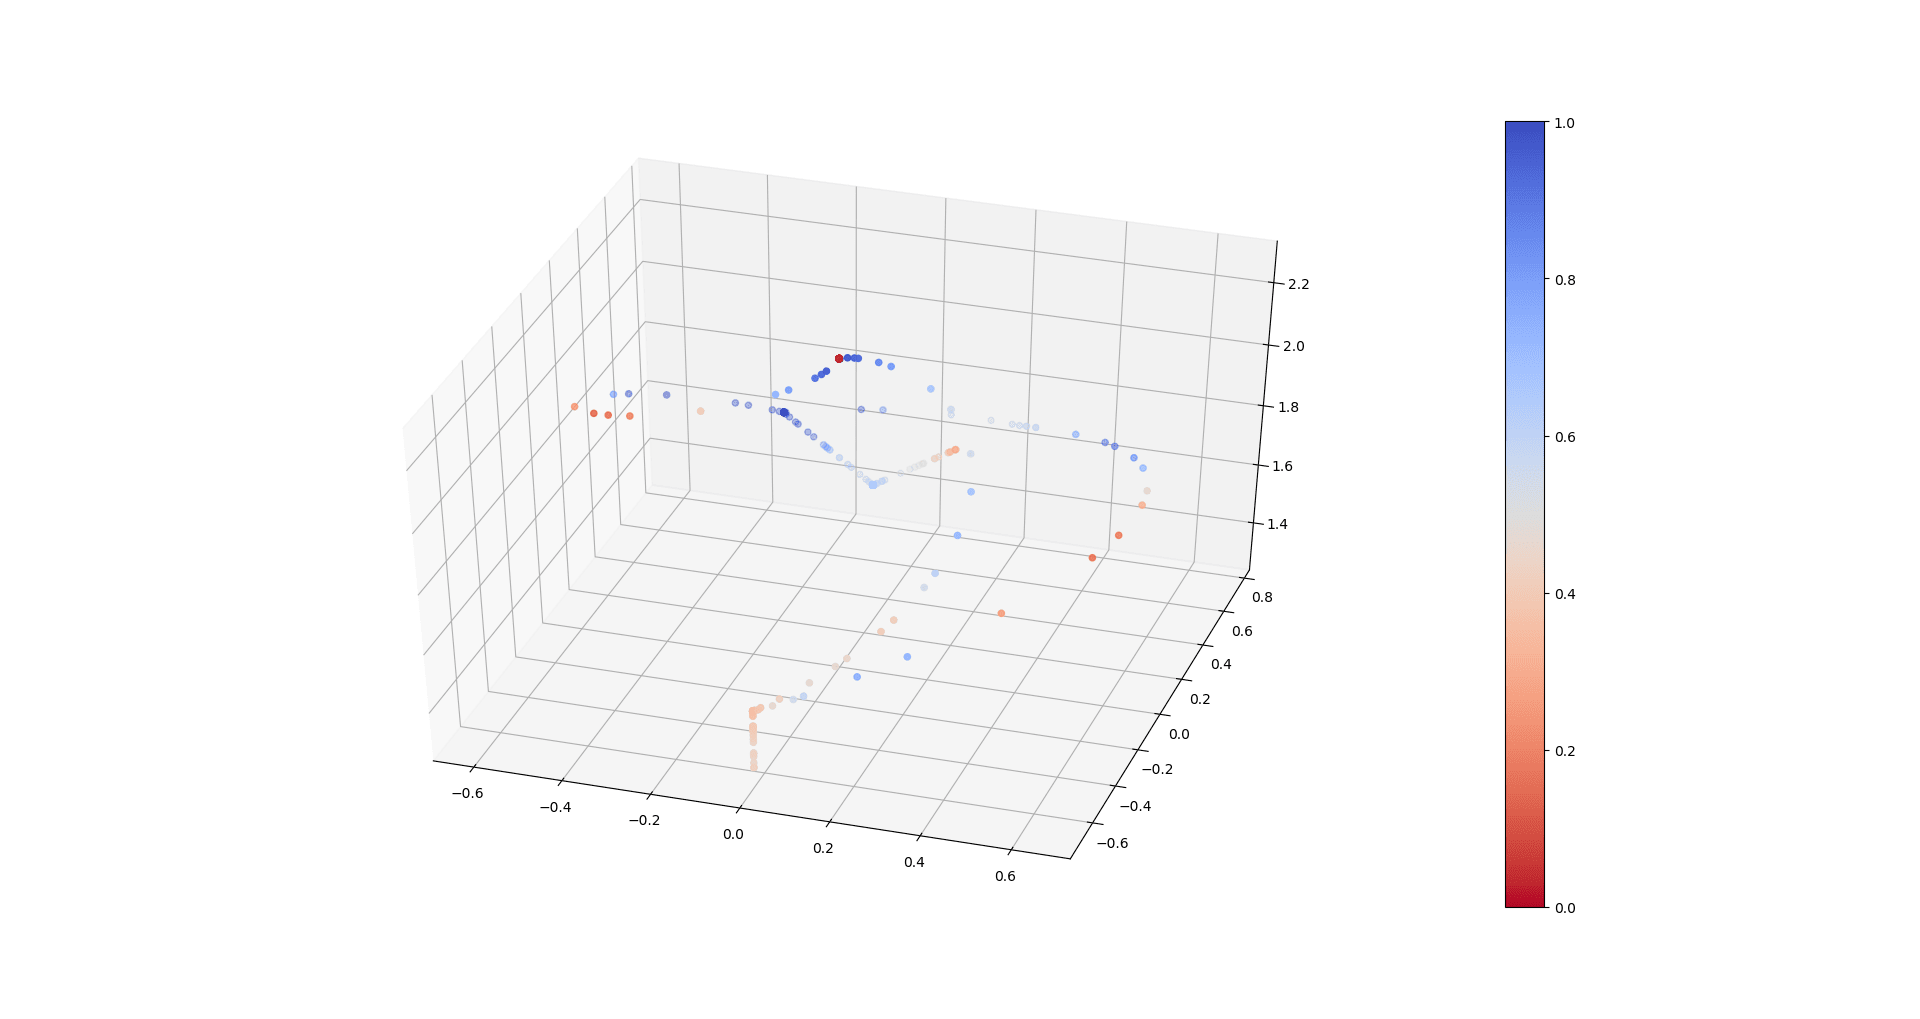
\includegraphics[width=10cm]{images/robot-planner1-manipulability-plot.png}\\
\caption{Plot the manipulability of the robot arm at sample points of the executed trajectory}
\end{figure}
\end{center}

The equation \ref{joint-limit-measure} calculates a joint limit measure which is multiplied with the manipulability measure and gives the dexterity measure.
From that equation we can conclude the following:
\begin{itemize}
\item If $q_i = q_{min}$ or $q_i = q_{max}$ then the exponential is equal to 1 which means that $\mathcal{L}_{q}$ and $\mathcal{D}$ are both 0, which means 
that the robot has \textbf{no dexterity at the boundary of the task space}.
\item If the value of $q_i$ is close to it's boundary value then the dexterity approaches 0. The how much close or far it is from the boundary (or in other words 
how fast the exponential term converges) depends on the parameter $\kappa$
\item The $q_{min}, q_{max}$ are calculated from the geometry of the task-space
\end{itemize}

For maximum dexterity at most points of a trajectory in a pivoting motion, the pivot sub-
taskspace (i.e. the space of all configurations of feasible pivot motions) must be fully within 
the robot’s whole reachable taskspace, otherwise only a small range of pivot movements will be 
feasible.



\subsection{Sampling methods}

The path planning algorithms that were mostly used in this thesis belong to the category of sampling methods. These methods use random functions to choose a sample from 
the configuration space or the state space. Sampling methods differ from the deterministic grid methods which, which discretize the whole space. Sampling methods are less 
computationally expensive than the grid methods, but they do not deliver optimal solutions like the latter.


\subsubsection{RRT Algorithms}

The \textbf{Rapidly-exploring Random Trees} algorithm is a sampling planning method that searches for an obstacle-free motion plan from an initial state $x_{init}$ to a set of goal states $\mathcal{X}_{goal}$. We refer to a set 
of goal states, because apart from the one desired goal state there can be other neighbor states that are within the allowed position and orientation tolerances.

\begin{algorithm}[H]
\SetAlgoLined
\ForEach{replanning attempt}{
	initialize vertices $V \leftarrow \lbrace x_{init} \rbrace$\;
	initialize edges $E \leftarrow \varnothing$\;
	initialize search tree $T \leftarrow (V,E)$\;
	\While{$time \leq maxPlanningTime$}{
		$x_{rand} \leftarrow$ getSampleStateFrom($\mathcal{X}$)\;
		$x_{nearest} \leftarrow$ getNearestNodeInTreeToState($T, x_{rand}$)\;
		$x_{new} \leftarrow$ findLocalPlanFromTo($x_{nearest}, x_{rand}$)\;
		\If{isPathCollisionFree($x_{nearest}, x_{rand}$)}{
			$V \leftarrow V \cup \lbrace x_{new} \rbrace $\;
			$E \leftarrow E \cup \lbrace (x_{nearest}, x_{rand}) \rbrace $\;
			\If{$x_{new} \in \mathcal{X}_{goal}$}{
				\Return SUCCESS and path plan $ T=(V,E) $ \;
			}
		}
	}
}
\Return FAILURE and $ T=(V,E) $ \;
\caption{RRT Algorithm}
\end{algorithm}

Other variations of the RRT Algorithm, which are also available in the OMPL library, included in the MoveIt library of ROS framework  are:
\begin{itemize}
	\item \textbf{TRRT} Transition-based RRT
	\item \textbf{BiTRRT} Bidirectional Transition-based RRT
	\item \textbf{RRT*}
	\item \textbf{RRTConnect} with is the default OMPL path planner in ROS
	\item \textbf{LBTRRT} Lower Bound Tree RRT
\end{itemize}


\subsubsection{PRM Algorithms}

The \textbf{Probabilistic Roadmap} (PRM) algorithm is a sampling planning method that constructs a roadmap representation of $\mathcal{C}_{free}$ \textbf{before searching} for a solution. After the roadmap is successfully built, then the algorithm searches 
for a solution using a traditional graph-based search algorithm. A very important aspect of this algorithm is how the sampling of the free configuration space will be done. The sampling is usually performed using a 
uniform distribution except from the regions close to objects where the sampling is more dense.

\begin{algorithm}[H]
\SetAlgoLined
initialize vertices $V \leftarrow \lbrace x_{init} \rbrace$\;
initialize edges $E \leftarrow \varnothing$\;
initialize roadmap graph $G \leftarrow (V,E)$\;
\For{$i = 1, \ldots , n$}{
	$x_{rand,i} \leftarrow$ getSampleStateFrom($\mathcal{X}$)\;
	$\mathcal{N}(x_{rand,i}) \leftarrow$ getKNearestNeighbors($G=(V,E), x_{rand,i}$)\;
	$V \leftarrow V \cup \lbrace x_{rand,i} \rbrace $\;
	\ForEach{$x \in \mathcal{N}(x_{rand,i})$}{
		\If{there is no edge between $x$ and $x_{rand,i}$}{
			\If{isPathCollisionFree($x_{nearest}, x_{rand,i}$)}{
				$E \leftarrow E \cup \lbrace (x_{rand,i}, x), (x, x_{rand,i}) \rbrace$
			}
		}
	}
}
\Return $G=(V,E)$
\caption{PRM roadmap construction (preprocessing phase)}
\end{algorithm}

Other variations of the PRM Algorithm, which are also available in the OMPL library, included in the MoveIt library of ROS framework  are:
\begin{itemize}
	\item \textbf{PRM*}
	\item \textbf{LazyPRM}
	\item \textbf{LazyPRM*}
\end{itemize}


\subsection{Pick and place algorithm}

% Help on using the algorithme package
% http://ftp.ntua.gr/mirror/ctan/macros/latex/contrib/algorithm2e/doc/algorithm2e.pdf 
\begin{algorithm}[H]
\SetAlgoLined
\ForEach{surgical tool}{
	\tcc{Plan the Pick pipeline}
	set grasp pose\;
	set pre-grasp approach\;
	set post-grasp retreat\;
	set posture of eef before grasp (open gripper)\;
	set posture of eef during grasp (closed gripper)\;
	\tcc{Plan the Place pipeline}
	set place location pose\;
	set pre-place approach\;
	set post-grasp retreat\;
	set posture of eef after placing object\;
	Plan pick and place paths\;
}
\caption{Pick and Place algorithm}
\end{algorithm}

If the pick and place algorithm targets small objects, such as cubes or spheres or other small convex objects then the path planning is straightforward. In the case where, the object to pick and place has at least one 
dimension that is bigger than the others like a rod or other long objects, such as the surgical tools, used in this thesis, then the path planning becomes more complicated, because of the almost certain collisions 
of the tool with the links of the rest of the robot (the link of the end-effector will probably not collide with the tool).